\documentclass{article}

% PACKAGES
\usepackage[margin=0.75in]{geometry}
\usepackage{amsmath}
\usepackage{amssymb}
\usepackage{graphicx}
\usepackage{subcaption}
\usepackage{float}

% TITLE
\title{Math 273A - Project 2}
\author{Eric Weise - A09642187}

\begin{document}
\maketitle

\begin{figure}[H]
    \caption{Starting obstacles}
    \centering
        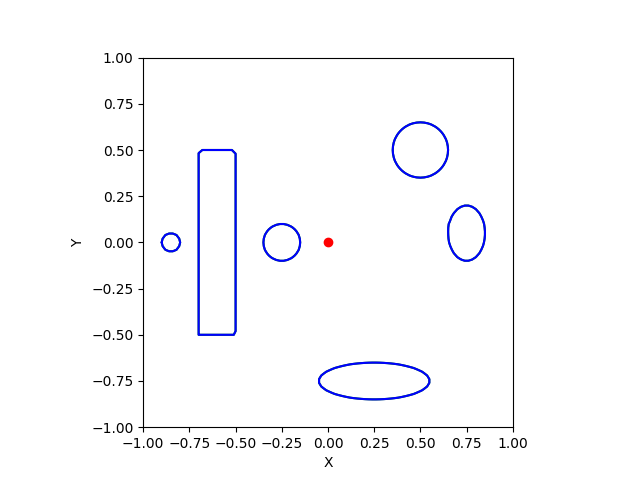
\includegraphics[width=0.5\textwidth]{part_a-levelset-0000.png}
\end{figure}


\section*{Part A}
\begin{figure}[H]
    \caption{Starting obstacles}
    \centering
        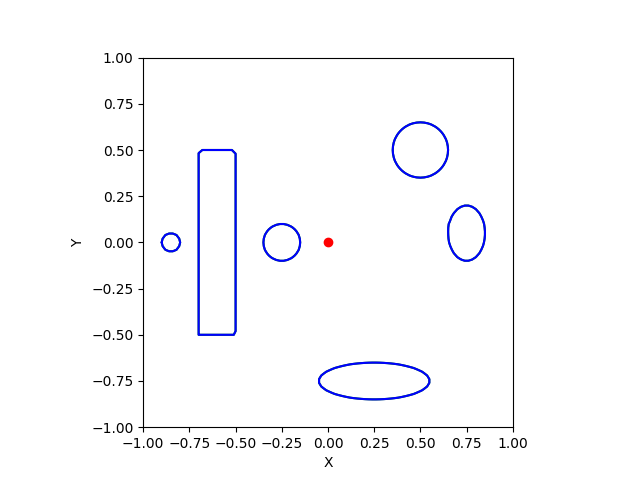
\includegraphics[width=0.5\textwidth]{part_a-levelset-0000.png}
\end{figure}

\begin{figure}[H]
    \caption{Levelset after 5 iterations}
    \centering
        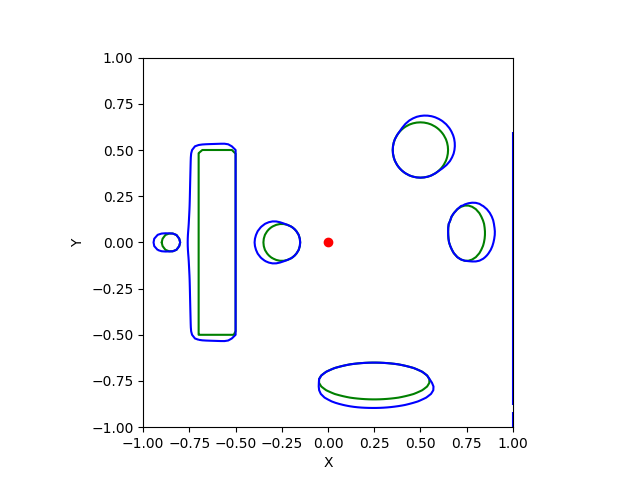
\includegraphics[width=0.5\textwidth]{part_a-levelset-0005.png}
\end{figure}

\begin{figure}[H]
    \caption{Levelset after 15 iterations}
    \centering
        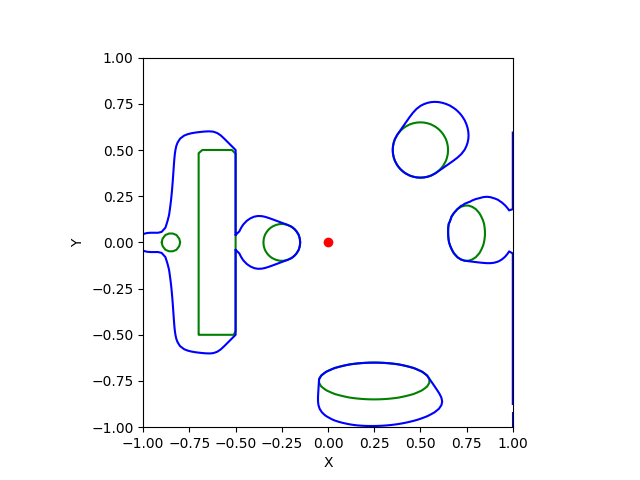
\includegraphics[width=0.5\textwidth]{part_a-levelset-0015.png}
\end{figure}

\begin{figure}[H]
    \caption{Levelset after 130 iterations}
    \centering
        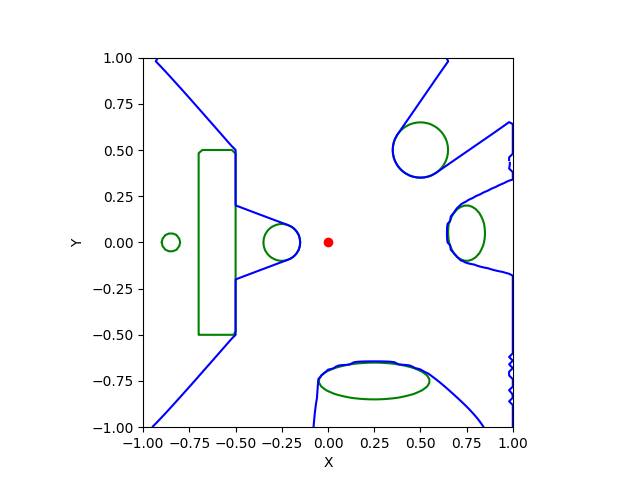
\includegraphics[width=0.5\textwidth]{part_a-levelset-0130.png}
\end{figure}



\newpage
\section*{Part B}
\begin{figure}[H]
    \caption{Starting obstacles}
    \centering
        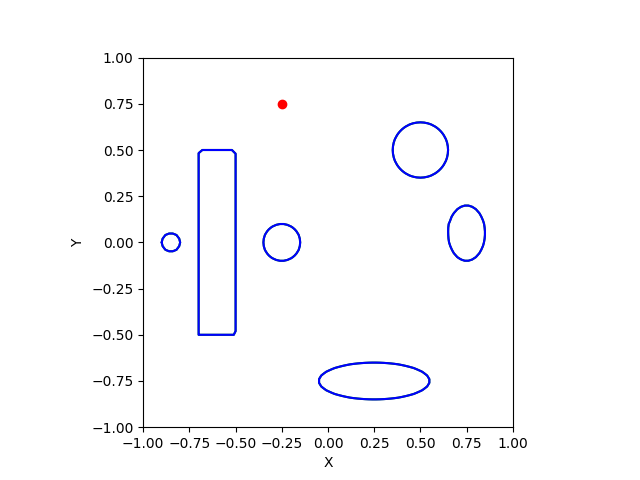
\includegraphics[width=0.5\textwidth]{part_b-levelset-0000.png}
\end{figure}

\begin{figure}[H]
    \caption{Levelset after 5 iterations}
    \centering
        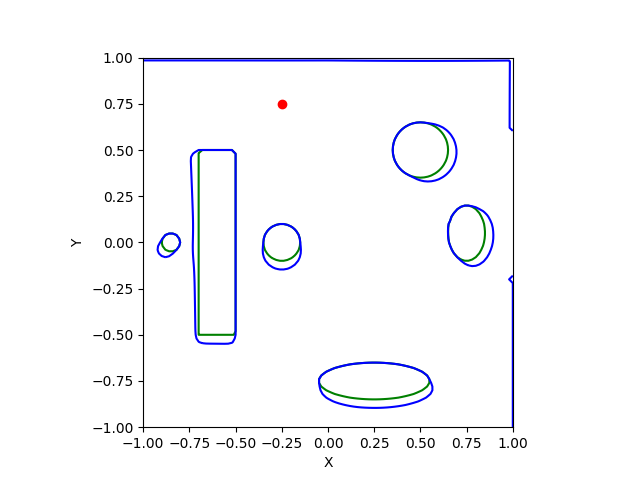
\includegraphics[width=0.5\textwidth]{part_b-levelset-0005.png}
\end{figure}

\begin{figure}[H]
    \caption{Levelset after 15 iterations}
    \centering
        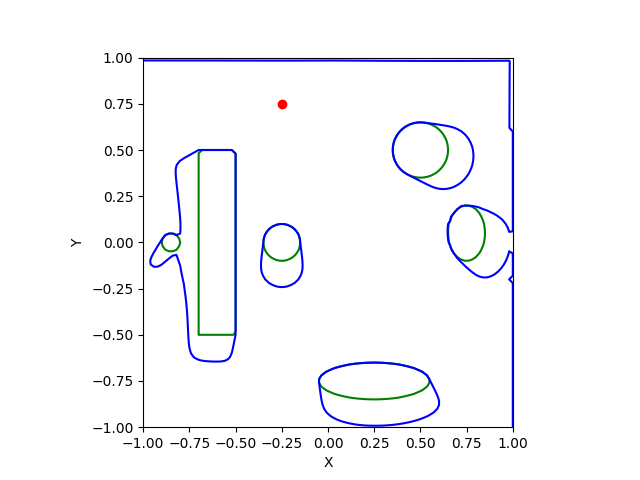
\includegraphics[width=0.5\textwidth]{part_b-levelset-0015.png}
\end{figure}

\begin{figure}[H]
    \caption{Levelset after 130 iterations}
    \centering
        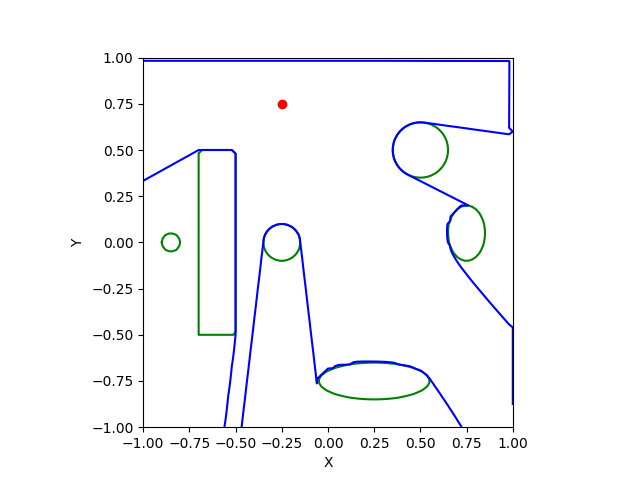
\includegraphics[width=0.5\textwidth]{part_b-levelset-0130.png}
\end{figure}




\newpage
\section*{Part C}
\begin{figure}[H]
    \caption{Regions visible to at least one eyepoint}
    \centering
        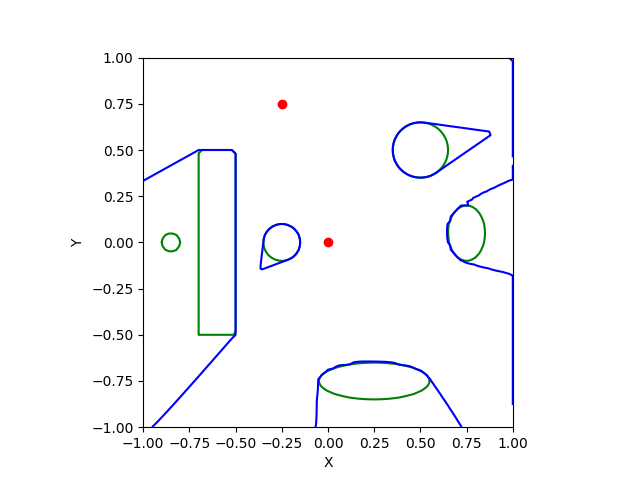
\includegraphics[width=0.5\textwidth]{part-c.png}
\end{figure}

\end{document}
